\chapter{Пример работы програмы}

\section{Поиск исполнителя}

Для этого воспользуетесь командой \texttt{/artist}.  Напишите, для
примера \texttt{/artist black sabbath}.  Бот в ответ присылает:

\begin{figure}[H]
  \centering
  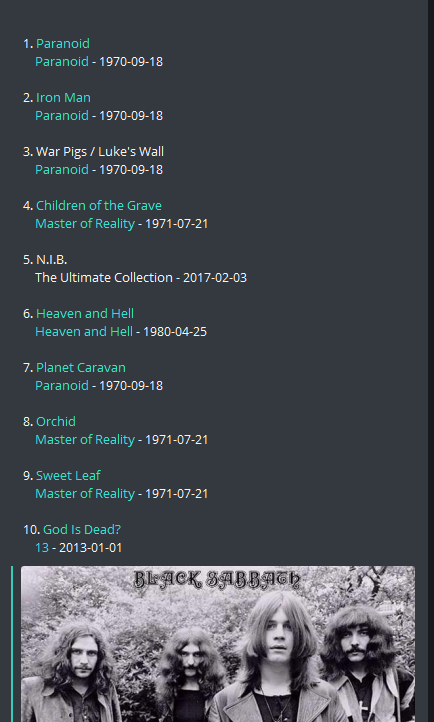
\includegraphics[width=8cm]{inc/img/artist.png}
\end{figure}

\section{Поиск альбома}

Для этого воспользуетесь командой \texttt{/album}.  Напишите, для
примера \texttt{/album black sabbath - paranoid}

\begin{figure}[H]
  \centering
  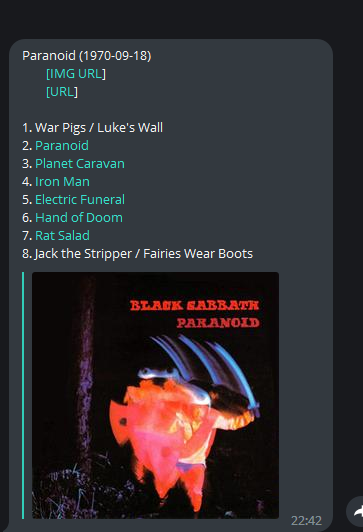
\includegraphics[width=8cm]{inc/img/album.png}
\end{figure}

\section{Поиск трека}

Для этого воспользуетесь командой \texttt{/track}.  Напишите, для
примера \texttt{/album black sabbath - paranoid}

\begin{figure}[H]
  \centering
  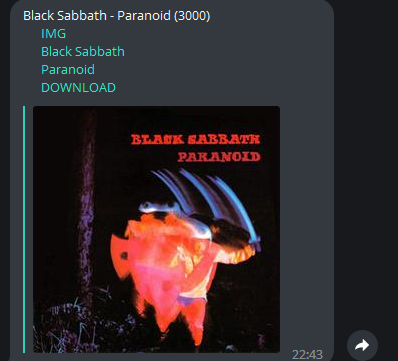
\includegraphics[width=8cm]{inc/img/track.png}
\end{figure}

Мне очень помогла следующая статья \cite{tg-bots}

Я думаю ты кру